%%%%%%%%%%%%%%%%%%%%%%%%%%%%%%%%%%%%%%%%%
% Beamer Presentation
% LaTeX Template
% Version 1.0 (10/11/12)
%
% This template has been downloaded from:
% http://www.LaTeXTemplates.com
%
% License:
% CC BY-NC-SA 3.0 (http://creativecommons.org/licenses/by-nc-sa/3.0/)
%
%%%%%%%%%%%%%%%%%%%%%%%%%%%%%%%%%%%%%%%%%

%----------------------------------------------------------------------------------------
%     PACKAGES AND THEMES
%----------------------------------------------------------------------------------------

\documentclass{beamer}
\usepackage[ngerman]{babel}


\mode<presentation> {

% The Beamer class comes with a number of default slide themes
% which change the colors and layouts of slides. Below this is a list
% of all the themes, uncomment each in turn to see what they look like.

%\usetheme{default}
%\usetheme{AnnArbor}
%\usetheme{Antibes}
%\usetheme{Bergen}
%\usetheme{Berkeley}
%\usetheme{Berlin}
%\usetheme{Boadilla}
%\usetheme{CambridgeUS}
%\usetheme{Copenhagen}
%\usetheme{Darmstadt}
%\usetheme{Dresden}
%\usetheme{Frankfurt}
%\usetheme{Goettingen}
%\usetheme{Hannover}
%\usetheme{Ilmenau}
%\usetheme{JuanLesPins}
%\usetheme{Luebeck}
\usetheme{Madrid}
%\usetheme{Malmoe}
%\usetheme{Marburg}
%\usetheme{Montpellier}
%\usetheme{PaloAlto}
%\usetheme{Pittsburgh}
%\usetheme{Rochester}
%\usetheme{Singapore}
%\usetheme{Szeged}
%\usetheme{Warsaw}

% As well as themes, the Beamer class has a number of color themes
% for any slide theme. Uncomment each of these in turn to see how it
% changes the colors of your current slide theme.

%\usecolortheme{albatross}
%\usecolortheme{beaver}
%\usecolortheme{beetle}
%\usecolortheme{crane}
%\usecolortheme{dolphin}
%\usecolortheme{dove}
%\usecolortheme{fly}
%\usecolortheme{lily}
%\usecolortheme{orchid}
%\usecolortheme{rose}
%\usecolortheme{seagull}
%\usecolortheme{seahorse}
%\usecolortheme{whale}
%\usecolortheme{wolverine}

%\setbeamertemplate{footline} % To remove the footer line in all slides uncomment this line
%\setbeamertemplate{footline}[page number] % To replace the footer line in all slides with a simple slide count uncomment this line

%\setbeamertemplate{navigation symbols}{} % To remove the navigation symbols from the bottom of all slides uncomment this line
}

\usepackage{graphicx} % Allows including images
\usepackage{booktabs} % Allows the use of \toprule, \midrule and
% \bottomrule in tables
\usepackage{listings}
\usepackage{parcolumns}
\usepackage[nocenter]{qtree}

\usepackage{eurosym}

%----------------------------------------------------------------------------------------
%     TITLE PAGE
%----------------------------------------------------------------------------------------

\title[Latex1]{Latex 1 -  Das bessere Word?} % The short title appears at the bottom of every slide, the full title is only on the title page

\author{Andreas Rist} % Your name
\institute[FSI] % Your institution as it will appear on the bottom of every slide, may be shorthand to save space
{
Uni Tübingen\\ % Your institution for the title page
\medskip
\textit{fsi@fsi.uni-tuebingen.de} % Your email address
}
\date{\today} % Date, can be changed to a custom date

\begin{document}

\begin{frame}
\titlepage % Print the title page as the first slide
\end{frame}

%----------------------------------------------------------------------------------------
%     PRESENTATION SLIDES
%----------------------------------------------------------------------------------------

%------------------------------------------------

\begin{frame}
\frametitle{Was is'n Latex bitte?}

\includegraphics[width=\linewidth]{pictures/latex_tree.png}
\begin{figure}
\centering


\includegraphics[width=0.7\linewidth]{pictures/latex_sexy.png}
\end{figure}
\end{frame}


\begin{frame}
\frametitle{Was ist Latex jetzt wirklich?}

\includegraphics[width=\linewidth]{pictures/reallatex.png}

\end{frame}

\begin{frame}
\frametitle{Was ist Latex jetzt wirklich?}
     Latex ist also eine freeware Version von Word?\pause $\Rightarrow$ Nein, besser!
     
\end{frame}


\begin{frame}
     \frametitle{Na was denn nu?}
     \begin{columns}[c] % The "c" option specifies centered vertical alignment while the "t" option is used for top vertical alignment
          
          \column{.2\textwidth} % Left column and width
     
\includegraphics[width=\textwidth]{pictures/texicon.png}
          \column{.1\textwidth} % Left column and width
     \Huge{$ \Rightarrow $}
          
          \column{.2\textwidth} % Right column and width
     
\includegraphics[width=\textwidth]{pictures/pdficon.png}
          
     \end{columns}
\begin{itemize}[<+->]
     \item Datei wird in *.tex geschrieben
     \item *.tex wird in eine PDF umgewandelt
\end{itemize}
\end{frame}

\begin{frame}
     \frametitle{Du hast umgewandelt gesagt?}
     \begin{itemize}[<+->]
          \item Ja! Du wirst einen Compiler brauchen
               \item mkLatex, \textbf{pdfLaTeX}, XeLaTeX and LuaLaTeX
               \item Unter Windows: MikTex
     \end{itemize}
\end{frame}




\begin{frame}
     \frametitle{Muss ich dann die Command-line benutzen?}
     Nein, keine Sorge! Es gibt tolle Editoren
     \begin{itemize}[<+->]
          \item Overleaf
          \item TexStudio
          \item Sublime 
          \item Atom
          \item vim
     \end{itemize}
\end{frame}

\begin{frame}
\frametitle{Wann kommen wir endlich zum Coden?}

\includegraphics[width=\linewidth]{pictures/anger.jpg}
\end{frame}

\begin{frame}[fragile]
     
\frametitle{Basis Gerüst}

\begin{columns}
     \column{.5\textwidth}\begin{block}{Gerüst}
          
          \begin{verbatim}
\documentclass[12pt]{scrartcl}
\usepackage[ngerman]{babel}
\usepackage[utf8]{inputenc}
% weitere imports...
\begin{document}
     (Inhalt)
\end{document}
     \end{verbatim}
     \end{block}
          \column{.45\textwidth}
          \textbf{Dokumenten Klassen}
          \begin{itemize}[<+->]
               \item article
               \item letter
               \item scrartcl 
               \item exam
          \end{itemize}\pause
     \textbf{Wichtigste Imports}
     \begin{itemize}[<+->]
          \item mathtools,amsthm,amssymb
          \item fancyhdr
          \item graphicx
     \end{itemize}
          
     \end{columns}
\end{frame}

\begin{frame}[fragile]
\frametitle{Header und Footer}
\begin{columns}
\column{.39\textwidth}

\begin{block}{}
     \begin{verbatim}
(...)
\usepackage{fancyhdr}
\pagestyle{fancy} 
\fancyhf{} 
\fancyhead[L]{Titel} 
\fancyhead[C]{}           
\fancyhead[R]{Name}           
\fancyfoot[C]{\thepage}  
\begin{document}
    (...)
\end{document}
          \end{verbatim}
     \end{block}
\column{0.5\textwidth}
\begin{figure}

\begin{example}

\includegraphics[width=\linewidth,trim= 0cm 20cm 0cm 0cm,]{pictures/asdf0.pdf}

\end{example}\end{figure}
\end{columns}

\end{frame}
%------------------------------------------------

\begin{frame}[fragile]
     \frametitle{Strukturierung und Nummerierung}
     \begin{columns}
          \column{.5\textwidth}
     \begin{block}{Kapitel}<1->
          \begin{verbatim}
\section{Sektion}
\subsection{SSektion}
\subsubsection{SSSektion}
\section*{Sektion}
          \end{verbatim}          
     \end{block}
     
\begin{block}{Aufzählung}<3->
     \begin{verbatim}
\begin{enumerate}
     \item Bla bla bla
     \item Mr Freeman
     \item here 
\end{enumerate}
     \end{verbatim}
     
\end{block}
\column{.45\textwidth}
\begin{example}

\includegraphics[width=\linewidth,trim=0cm 20cm 10cm 0cm]{pictures/asdf2.pdf}
\end{example}

\end{columns}
\end{frame}

\begin{frame}[fragile]
     \frametitle{Strukturierung und Nummerierung}
     \begin{columns}
     \column{.45\textwidth}
     
     \begin{block}{Stichpunkte}
          \begin{verbatim}
\begin{itemize}
    \item Bla bla bla
    \item Mr Freeman
    \item here 
\end{itemize}
          \end{verbatim}
      \end{block}
      \column{.45\textwidth}
      \pause
      \begin{example}
      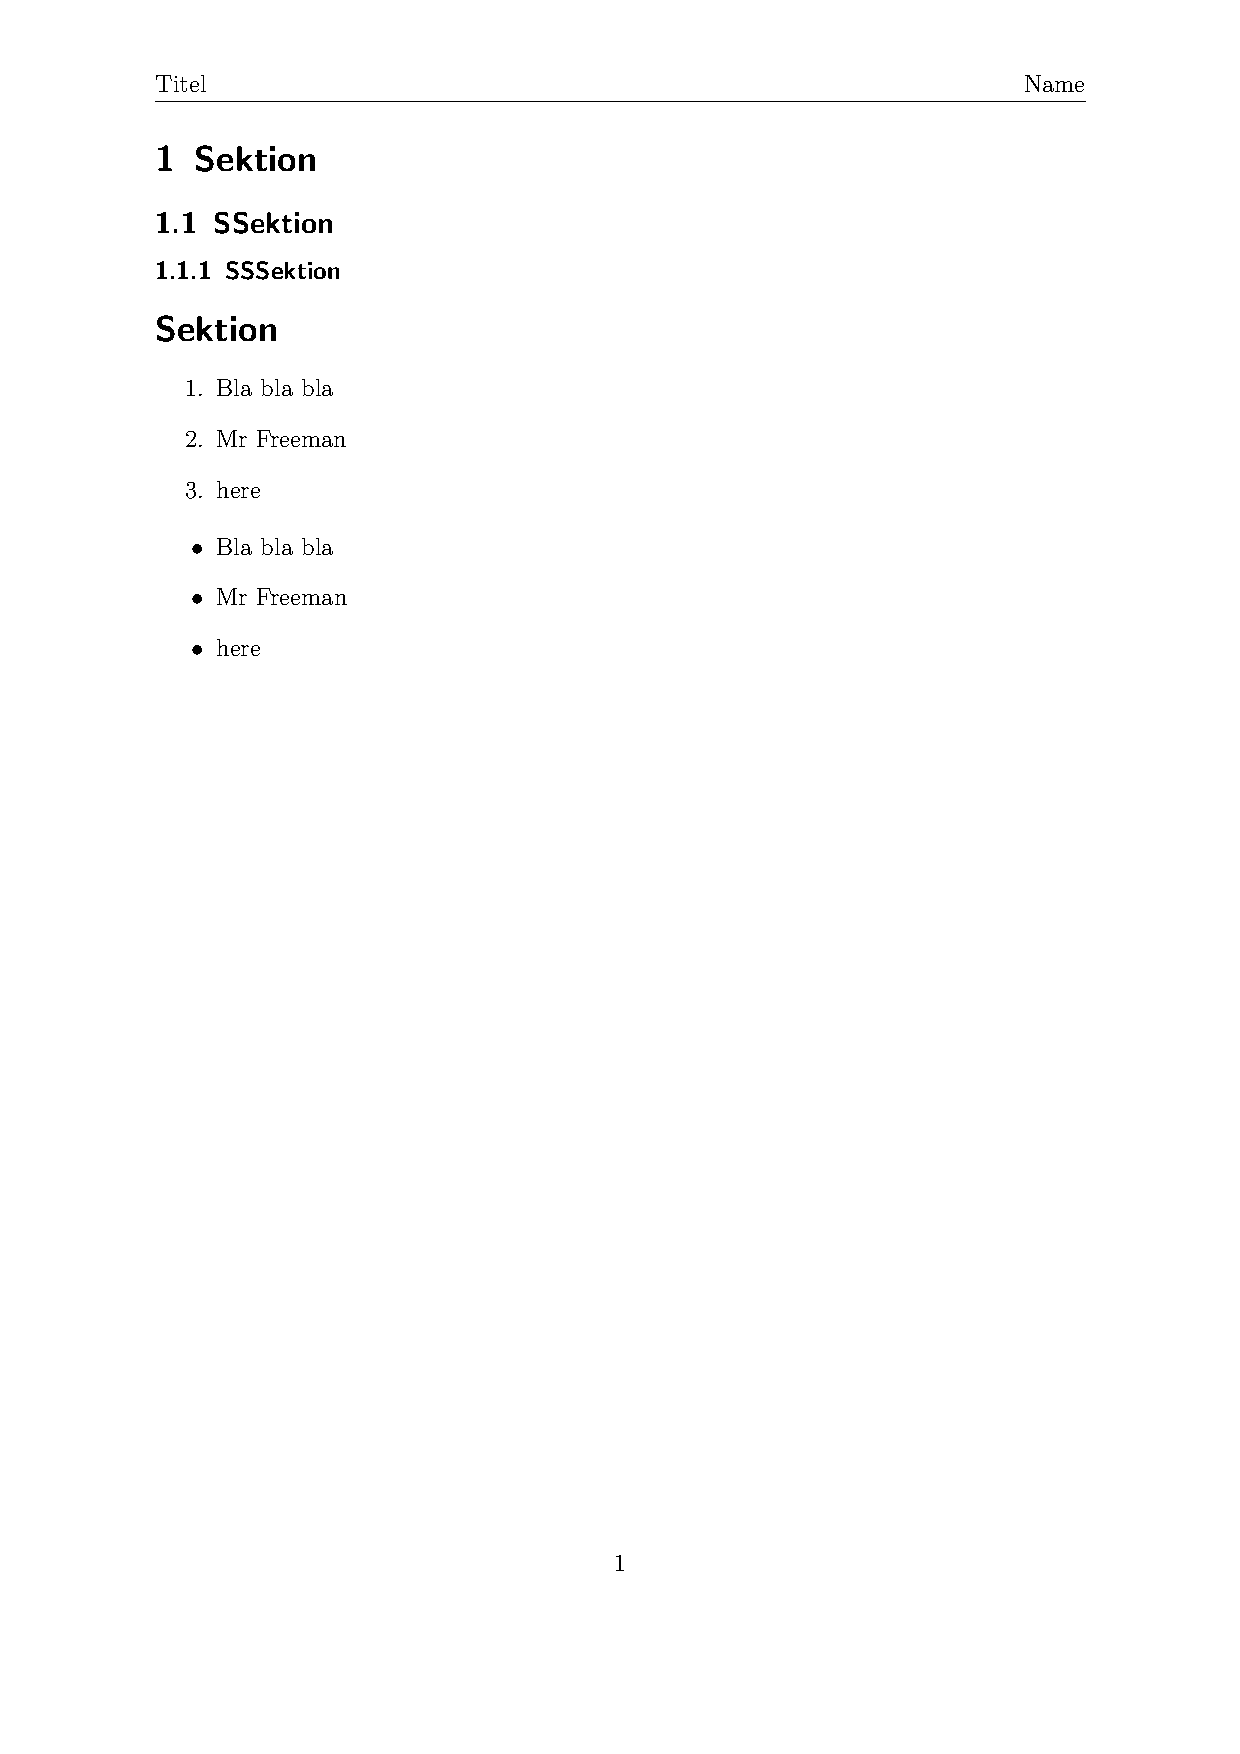
\includegraphics[width=\linewidth,trim=0cm 17cm 10cm 0cm]{pictures/asdf3.pdf}
      \end{example}
     
     
     \end{columns}

\end{frame}

\begin{frame}[fragile]
     \frametitle{Euch gefällt die Nummerierung nicht?}
     
     \begin{columns}
     \column{0.45\textwidth}
     \begin{block}{andere Nummerierungen}
               
          \begin{verbatim}
\usepackage{enumerate}
\usepackage[shortlabels]
{enumitem}
(...)
\begin{enumerate}[a)]
    \item
     \item 
     \item[5]
\end{enumerate}
          \end{verbatim}
          \end{block}

     \column{0.45\textwidth}
          \begin{example}
                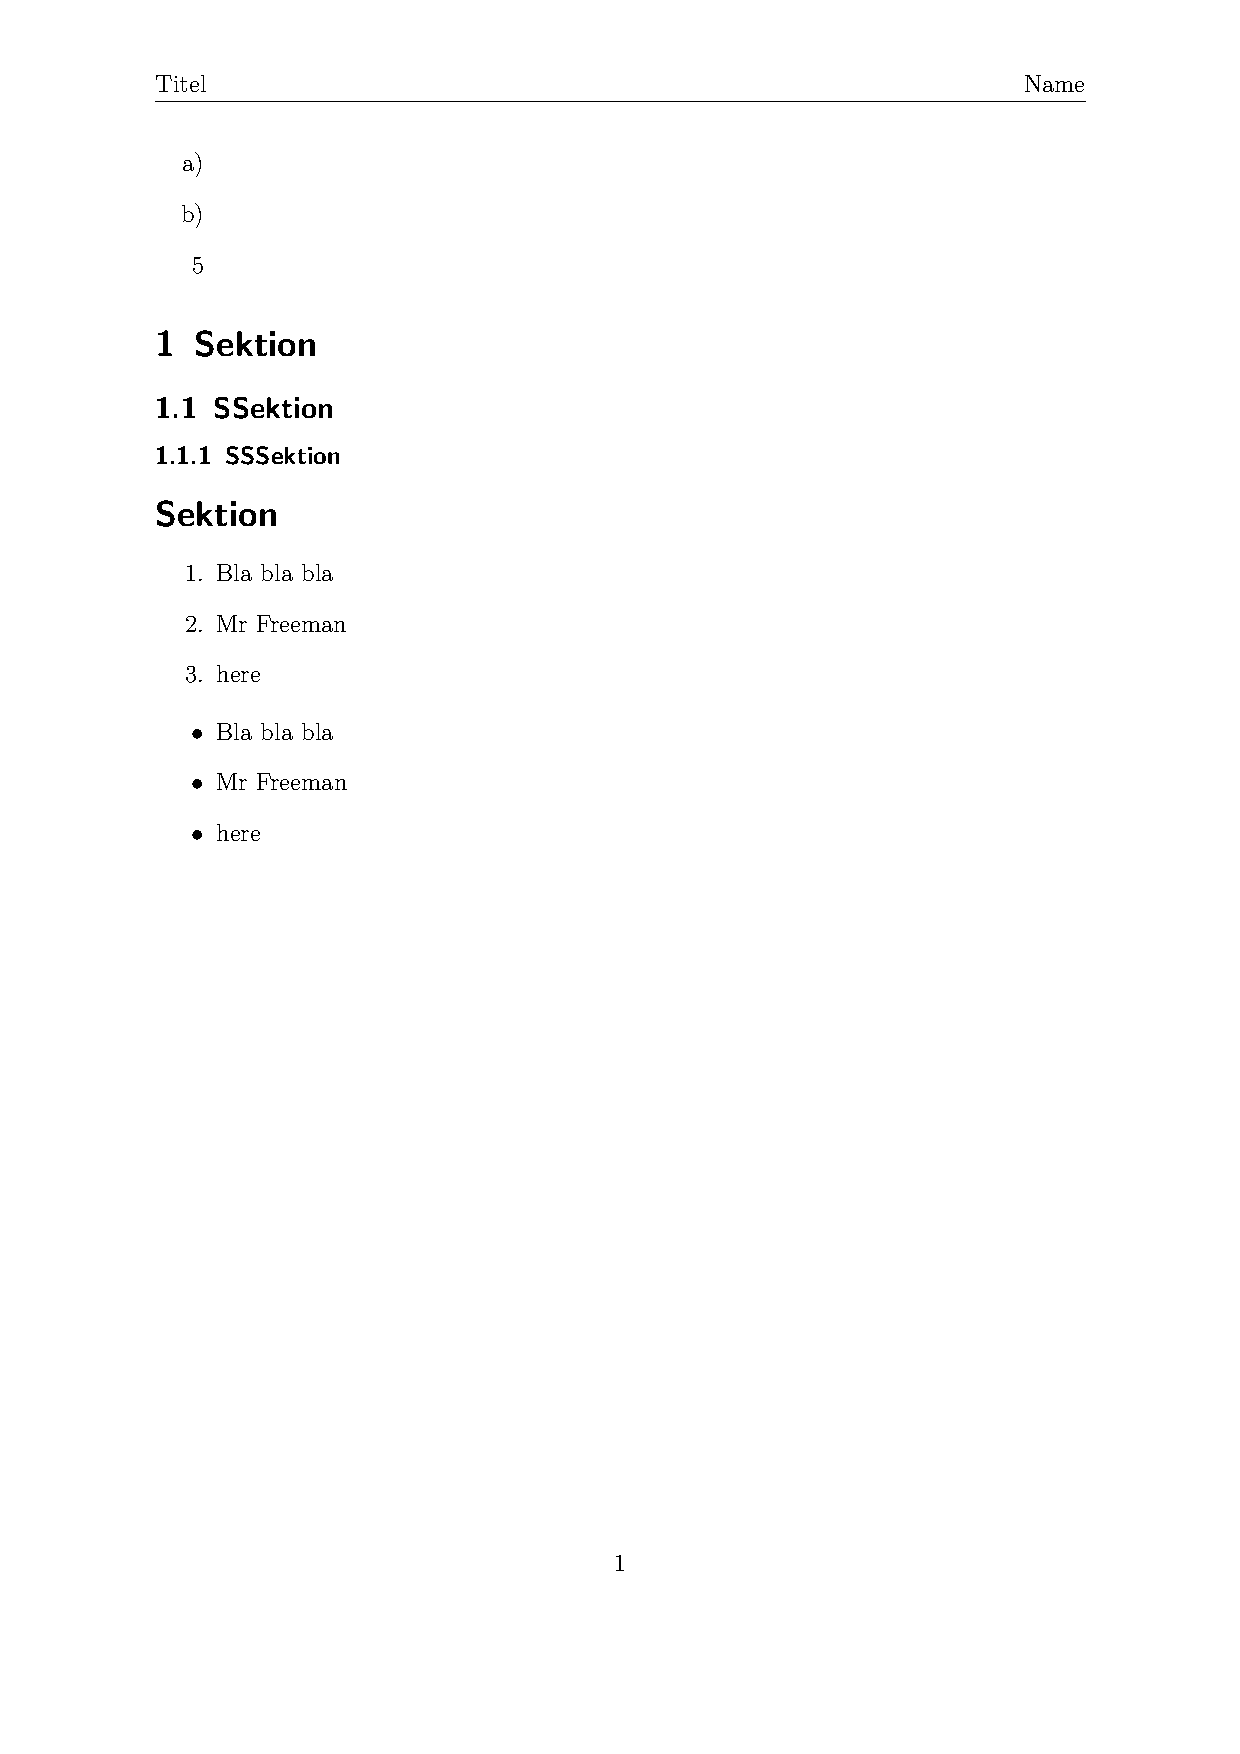
\includegraphics[width=\linewidth,trim= 0cm 10cm 0cm 0cm]{pictures/asdf4.pdf}
          \end{example}
     \end{columns}



\end{frame}

\begin{frame}[fragile]
\frametitle{Wie füge ich Bilder ein?}
\begin{block}{}
     \begin{verbatim}
\usepackage{graphicx}
(...)

\includegraphics[width=\linewidth]{pictures/balu.png}
     \end{verbatim}
\end{block}
\begin{example}
     
\includegraphics{pictures/balu.jpg}
\end{example}

\end{frame}

\begin{frame}[fragile]
\frametitle{Wie gebe ich Bildern Untertitel?}
\begin{block}{}
     \begin{verbatim}
\begin{figure}
\centering

\includegraphics{pictures/balu.jpg}
\caption{Balu}
\end{figure}
     \end{verbatim}
     
\end{block}
\begin{example}\begin{figure}
     \centering
     
\includegraphics[height=.3\textheight]{pictures/balu.jpg}
     \caption{Balu}
\end{figure}

\end{example}
\end{frame}

\begin{frame}[fragile]
     \frametitle{Tabellen}
\begin{example}
     \begin{table}
          \begin{tabular}{l||c |r}
               Nummer& Schulden & Person der Schuld \\\hline
               1& 10\euro & Mirco \\
               2& 100\euro &Fachschaft\\
               3&1000\euro & Kuchen\\
          \end{tabular}
     \caption{Schuldentablle}

     \end{table}
\end{example}

\end{frame}

\begin{frame}[fragile]
\frametitle{Tabellen2}
     \begin{block}{}
          \begin{verbatim}
\begin{table}
    \begin{tabular}{l||c |r}
        Nummer& Schulden & Person der Schuld \\\hline
        1& 10\euro & Mirco \\
        2& 100\euro &Fachschaft\\
        3&1000\euro & Kuchen\\
    \end{tabular}
\caption{Schuldentablle}
\end{table}
               
          \end{verbatim}
     \end{block}
\end{frame}

\begin{frame}
\frametitle{Mathematikumgebungen}
\begin{itemize}[<+->]
\item Inline würde man einfach $\sum_{1}^{100}i=5050$ schreiben
\item Aber das ist nicht schön, darum schreiben wir lieber
\[ \sum_{1}^{100}i=\frac{100(100+1)}{2}=5050 \]
in einer neuen Zeile, damit unsere tolle Formel auch auffällt
\item Naja, aber eigentlich müssen wir auch manchmal Formeln umformen
\begin{align*}
\sum_{k=1}^{n}2k&=2\cdot\sum_{k=1}^{n} k\\
&=2\cdot\frac{n(n+1)}{2}\\
&=n(n+1) = n^2+n
\end{align*}
\end{itemize}

\end{frame}

\begin{frame}[fragile]
\frametitle{Hinter der Mathemagie!}
\begin{block}{}
\begin{verbatim}
 $\sum_{1}^{100}i=5050$
\end{verbatim} 
\end{block}
\pause
\begin{example}
$\sum_{1}^{100}i=5050$
\end{example}
\pause
\begin{block}{}
\begin{verbatim}
\[ \sum_{1}^{100}i=\frac{100(100+1)}{2}=5050 \]
\end{verbatim}
\end{block}
\pause
\begin{example}
\[ \sum_{1}^{100}i=\frac{100(100+1)}{2}=5050 \]
\end{example}

\end{frame}
\begin{frame}[fragile]
\frametitle{Align Umgebung}
\begin{block}{}
\begin{verbatim}
\begin{align*}
    \sum_{k=1}^{n}2k&=2\cdot\sum_{k=1}^{n} k\\
                    &=2\cdot\frac{n(n+1)}{2}\\
                    &=n(n+1) = n^2+n
\end{align*}
\end{verbatim}
\end{block}
\begin{example}
\begin{align*}
    \sum_{k=1}^{n}2k&=2\cdot\sum_{k=1}^{n} k\\
                    &=2\cdot\frac{n(n+1)}{2}\\
                    &=n(n+1) = n^2+n
\end{align*}
\end{example}
\end{frame}
\begin{frame}[fragile]
\frametitle{Hast du Klammern gesagt?}
Natürlich gibt es probleme beim Klammern setzen!\\
\[f(x)=(\sum_{k=1}^{n}\underbrace{\frac{5(x+3)}{5}}_{=x+3})+g(x)\]\pause
"HEY! Das sieht blöd aus!"\pause Keine Sorge das geht besser!\\
\[f(x)=\left(\sum_{k=1}^{n}\underbrace{\frac{5(x+3)}{5}}_{=x+3}\right)+g(x)\]\pause
\begin{example}
\begin{verbatim}
\[f(x)=\left(
\sum_{k=1}^{n}\underbrace{\frac{5(x+3)}{5}}_{=x+3}
\right)
+g(x)\]
\end{verbatim}
\end{example}


\end{frame}

\begin{frame}[fragile]
\frametitle{ja gut... aber }
"Was ist mit dem Zeug, dass sie über die Gleichzeichen schreiben?"\pause
Meinst du vielleicht?
\[(a+b)^2\overset{ausm.}{=} a^2+2ab+b^2\]
\begin{example}
\begin{verbatim}
\[(a+b)^2\overset{ausm.}{=} a^2+2ab+b^2\]
\end{verbatim}
\end{example}\pause 
\begin{alertblock}{Aufgabe}
\[\int_{a}^{b}\left( f(x)+g(x)\right)dx=\int_{a}^{b}f(x)dx+\int_{a}^{b}g(x)dx\]
\end{alertblock}

\end{frame}

\begin{frame}[fragile]
\frametitle{Graphen und Bäume?}
\begin{itemize}[<+->]
\item yWorks yed
\begin{itemize}
\item[+] Einfach zu Bedienen 
\item[+] Sehr mächtig
\item[-] man bekommt nur SVG oder anderes Bildformat
\end{itemize}
\item FSM Designer
\begin{itemize}
\item http://madebyevan.com/fsm/
\item[+] yeah man bekommt tex code
\item[-] code nicht gut lesbar
\end{itemize}
\end{itemize}\pause
"Hey ich will das selber machen!"

\end{frame}
\begin{frame}[fragile]
\frametitle{ja gut, ja gut}
"Welches Package brauche ich?"\pause
\begin{itemize}[<+->]
\item \textbf{qtree}\\
\Tree [.VP \qroof{this}.DP [.V$'$ is \qroof{a tree}.DP ] ]
\begin{verbatim}
\Tree [.VP \qroof{this}.DP [.V$'$ is \qroof{a tree}.DP ] ]
\end{verbatim}
\item \textbf{tikz}
\end{itemize}

\end{frame}

\begin{frame}
\frametitle{Pseudocode?}
\begin{itemize}[<+->]
\item verbadim
\begin{itemize}
\item klein und gut!
\end{itemize}
\item lstlisting
\begin{itemize}
\item eher geignet für Code der direkt aus einem File importiert wird
\item Syntaxhighlighting
\item Konfigurationsmöglichkeiten ohne Ende
\end{itemize}
\item pseudocode
\begin{itemize}
\item Sehr gut für Algorithmen
\end{itemize}
\end{itemize}
\end{frame}

\begin{frame}
\frametitle{Wie siehts aus? Gibt es keine Tricks?}
Klar!
\begin{itemize}
\item https://www.tablesgenerator.com/
\item http://detexify.kirelabs.org/classify.html
\item https://mathpix.com/
\end{itemize}
\end{frame}




\end{document} 